\documentclass[aspectratio=169,mathserif]{beamer}

\usepackage[utf8]{inputenc}
\usepackage{graphicx}
\usepackage{tikz}
\usepackage{pgfplots}
\pgfplotsset{compat=newest}

\useoutertheme[numbering=fraction]{metropolis}
\useinnertheme{metropolis}
\usefonttheme{metropolis}
\usecolortheme{default}
\setbeamertemplate{title page}{
\begin{minipage}[b][\paperheight]{\textwidth}
\ifx\inserttitlegraphic\@empty\else\usebeamertemplate*{title graphic}\fi
\vfill%
\ifx\inserttitle\@empty\else\usebeamertemplate*{title}\fi
\ifx\insertsubtitle\@empty\else\usebeamertemplate*{subtitle}\fi
\usebeamertemplate*{title separator}
\ifx\beamer@shortauthor\@empty\else\usebeamertemplate*{author}\fi
\ifx\insertinstitute\@empty\else\usebeamertemplate*{institute}\fi
\ifx\insertdate\@empty\else\usebeamertemplate*{date}\fi
\vfill
\vspace*{1mm}
\end{minipage}
}

%%% Local Variables:
%%% mode: latex
%%% TeX-master: t
%%% End:

\usepackage{appendixnumberbeamer}
\usepackage{FiraSans}

\title{Wealth Inequality through the Lens of the Aiyagari Model}
\author{Fabian Greimel}
\date{June 2025}

\begin{document}

\frame{\titlepage}

% \begin{frame}{Learning Objectives}
% \begin{itemize}
%     \item Understand extensions of the Aiyagari model used to match U.S. wealth inequality
%     \item Evaluate the roles of tax policy, earnings risk, and portfolio heterogeneity
%     \item Critically assess model calibration and mechanisms
%     \item Propose and reason about additional model features
% \end{itemize}
% \end{frame}

% \begin{frame}{Lecture Structure}
% \begin{enumerate}
%     \item Recap and motivation
%     \item Model comprehension (discussion)
%     \item Deep-dive: mechanisms and calibration
%     \item Creative extensions
%     \item Wrap-up and outlook
% \end{enumerate}
% \end{frame}

\begin{frame}{Figure 1}
    \centering
    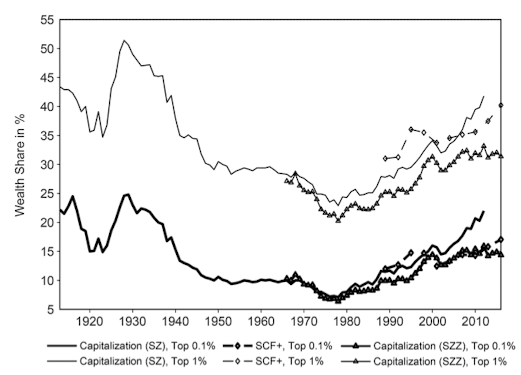
\includegraphics[scale = 0.5]{HKS_Fig_1.png}
\end{frame}

\begin{frame}{About Figure 1: Wealth inequality over time}

    \begin{itemize}
        \item problems with surveys
        \begin{itemize}
            \item sample size too small to get top 0.1\%
            \item truthful responses?
            \item short time series
        \end{itemize}
        \item SCF+ uses Forbes 400
        \item capitalization method: use past administrative data on earnings
    \end{itemize}
    
\end{frame}

\begin{frame}{Figure 6}
    \centering
    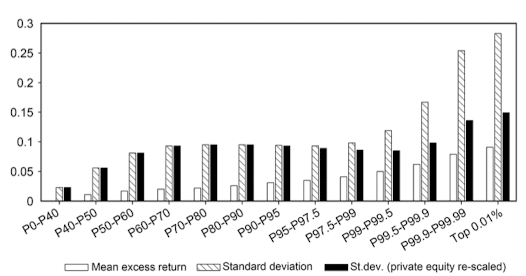
\includegraphics[scale = 0.5]{HKS_Fig_6.png}
\end{frame}

\begin{frame}{About Figure 6: Heterogenous returns on wealth}

    \begin{itemize}
        \item excess return: relative to risk-free rate
        \item different portfolios along the distribution (first lecture)
       
        \item excess return and risk rise with wealth level (cash vs stocks)
        \begin{itemize}
         \item Finance view: expectected return compensates high risk
        \end{itemize}
    \end{itemize}
    
\end{frame}


\begin{frame}{Extensions over simple Aiyagari from lecture}
    \begin{itemize}
        \item more complicated income process
        \item (progressive) taxes
        \item heterogenous returns on wealth (level $r(a)$ and risk $\sigma(a)$)
        \item \textcolor{gray}{heterogenous discount rates (cf Krusell \& Smith)}
    \end{itemize}
    
\end{frame}




% \begin{frame}{The Household Problem in Aiyagari (1994)}
% The household maximizes expected discounted utility:
% \[
% V(a, y) = \max_{c, a'} \left\{ u(c) + \beta \mathbb{E}[V(a', y')] \right\}
% \]
% subject to the budget constraint:
% \[
% c + a' = (1 + r) a + y
% \]
% and borrowing constraint:
% \[
% a' \geq \underline{a}
% \]
% where
% \begin{itemize}
%     \item $a$ is current assets,
%     \item $y$ is labor income,
%     \item $r$ is the interest rate,
%     \item $c$ is consumption,
%     \item $\beta$ is the discount factor,
%     \item $u(\cdot)$ is the utility function.
% \end{itemize}
% \end{frame}

\begin{frame}{Recall: Aiyagari}
    \begin{align*}
    V(a, y) &= \max_{c, a'} \left\{ u(c) + \beta \mathbb{E}[V(a', y')] \right\} \\
    &\begin{aligned} \text{s.t. } & c + a' = (1 + r) a + y
        \\
       % &\textcolor{red}{r = r(a) + \sigma(a) \cdot x} \\
        &y \sim \text{some Markov Chain} \\
        &a' \geq \underline{a}
    \end{aligned}
    \end{align*}
    where
    \begin{itemize}
        \item $a$ is current assets,
        \item $y$ is risky labor income,
        \item $r$ is the interest rate,
        \item $\beta$ is the discount factor.
    \end{itemize}
\end{frame}

\begin{frame}{Aiyagari with Heterogeneous Returns}
    \begin{align*}
    V(a, y) &= \max_{c, a'} \left\{ u(c) + \beta \mathbb{E}[V(a', y')] \right\} \\
    &\begin{aligned} \text{s.t. } & c + a' = (1 + r) a + y
        \\
        &\textcolor{red}{r = r(a) + \sigma(a) \cdot x} \\
        &y \sim \text{some Markov Chain} \\
        &a' \geq \underline{a}
    \end{aligned}
    \end{align*}
    where
    \begin{itemize}
        \item $r(a)$ is the deterministic return depending on wealth level,
        \item $\sigma(a)$ is the wealth-dependent return volatility,
        \item $x$ is an independent shock to returns
    \end{itemize}
\end{frame}

\begin{frame}{Table 2}
    \centering
    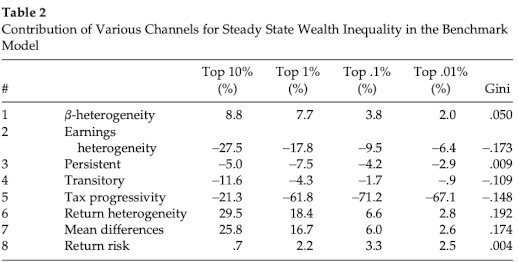
\includegraphics[scale = 0.7]{HKS_Tab_2.png}
\end{frame}

\begin{frame}{About Table 2: Drivers of wealth inequality}

    \begin{itemize}
        \item Gini is old-school
        \item interpret numbers
        \item how do rows 6--8 relate to each other (effects non-linear)
        \item Why might more risk reduce inequality?
        \item idea of persistent vs transitory
    \end{itemize}

\end{frame}

\begin{frame}{Table 4}
    \centering
    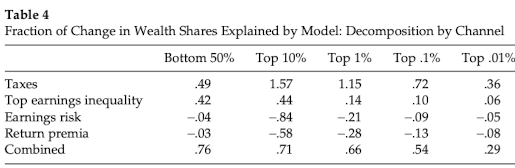
\includegraphics[scale = 0.7]{HKS_Tab_4.png}
\end{frame}
\begin{frame}{Figure 8}
    \centering
    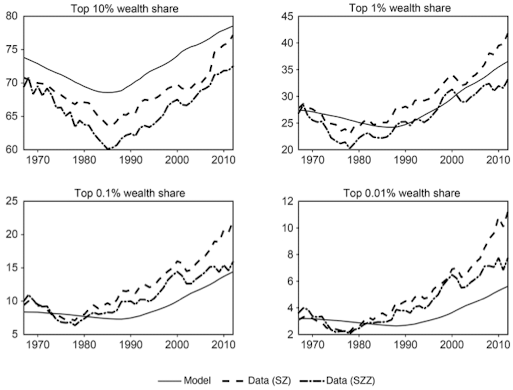
\includegraphics[scale = 0.5]{HKS_Fig_8.png}
\end{frame}

% \begin{frame}{Mechanisms and Calibration}
% \textbf{Discussion:}
% \begin{itemize}
%     \item Tax progressivity, asset prices, capital share
%     \item Calibration choices and empirical grounding
%     \item Data sensitivity
% \end{itemize}
% \end{frame}

\begin{frame}{Extensions}
    \begin{itemize}
        \item What other channels determine wealth inequality?
        \item How would you add them to the model?
    \end{itemize}
\end{frame}

\begin{frame}{Wrap-Up and Reflections}
\begin{itemize}
    \item Recap: mechanisms driving inequality in the model
    \item Next time: wealth tax
    %\item Final Q\&A
\end{itemize}
\end{frame}

\end{document}